\documentclass[addpoints]{exam}
\usepackage{amsmath,enumitem,wrapfig,amsfonts}
\usepackage{cancel}
\usepackage{tikz}
\usepackage{listings}
\newcommand{\StudentName}{Sabarno Saha - 22MS037}
\newcommand{\AssignmentName}{Assignment 02}
\pagestyle{headandfoot}
\runningheadrule
\runningheader{PH2101}{\StudentName}{\AssignmentName}
\firstpagefooter{}{}{\thepage}
\runningfooter{}{}{\thepage}
\usepackage[breakable]{tcolorbox}
\usepackage{parskip} % Stop auto-indenting (to mimic markdown behaviour)
% \usepackage{minted}
\printanswers
% \newminted{python}{fontfamily=courier,obeytabs,showtabs,breaklines,mathescape,linenos,numbersep=5pt,frame=single,numbersep=5pt,xleftmargin=0pt,fontsize=\scriptsize,frame=single,linenos=true,framesep=2mm,showspaces=false}
\lstset{
  basicstyle =\ttfamily,
  columns = fullflexible,
  frame=single,
  breaklines=true,
  postbreak=\mbox{\textcolor{red}{$\hookrightarrow$}\space},
}
\begin{document}

%starting page
\par\textbf{IISER Kolkata} \hfill \textbf{Assignment 2}
\vspace{3pt}
\hrule
\vspace{3pt}
\begin{center}
        \LARGE{\textbf{PH2101 : Waves and Optics}}
\end{center}
\vspace{3pt}
\hrule
\vspace{4pt}
\textbf{Sabarno Saha}, \textbf{22MS037}\hfill \today
\vspace{20pt}
\bigskip
%starting page end
\begin{questions}
\question 
\textbf{Question 1}
Consider a beaded string of $N$ beads each of mass $m$ (approximated as a long chain of spring-
mass system as shown in the figure). The beads are uniformly placed on the string and the
string has a uniform tension $T$ . The horizontal distance between any two beads in equilibrium
is a. The unstretched lengths of the springs are negligible.\\ \\ 
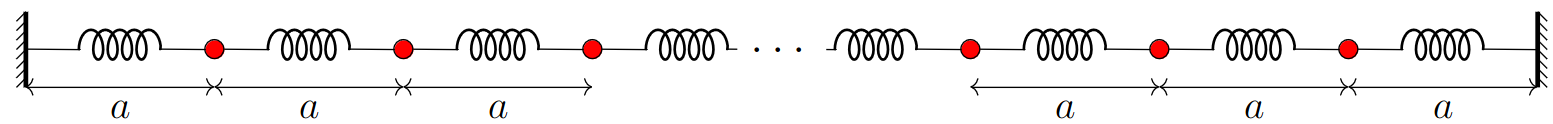
\includegraphics[width = 6.0in]{q1.png}\\ 
(a) Find the equation of the motion of $n^{th}$ bead for the longitudinal mode of vibration
\begin{solution}
 
\end{solution}
(b) Assuming normal mode vibration, find the normal mode frequency $\omega_m$ for $m^{th}$ mod
\begin{solution}
 
\end{solution}
(c) Find the amplitudes of the beads in $m^{th}$ mode ($A^{(m)}_n$ using the notation used in the class).
\begin{solution}
 
\end{solution}
(d) Plot the dispersion relation $\omega$ versus $k$.
\begin{solution}
 
\end{solution}
(e) Check whether we have $\omega_{N+2} = \omega_N$?
\begin{solution}
 
\end{solution}
(f) Check whether we have $A^{(N +2)}_n = A^{(N)}_n$?
\begin{solution}
 
\end{solution}
(g) Qualitatively plot $A^{(1)}_n$ and $A^{(N)}_n$ for all $n$.
\begin{solution}
 
\end{solution}

\question\textbf{Question 2}
Consider two pendulums, $a$ and $b$, with the same string length $L$, but with different bob masses, $M_a$ and $M_b$. They are coupled by a spring of spring constant $K$ which 
is attached to the bobs. Assuming small angle oscillations, \\ \\ 
(a) Find the equations of motion using angles of the pendulums (w.r.t. the vertical) as dynamical variables.
\begin{solution}
    Let the coupled pendula be shifted by $\theta_a$ and $\theta_b$ for $M_a$ and $M_b$ respectively
    Then for the mass $M_a$ we have the torque to be under small angles of displacement 
    \begin{align*}
        &\Gamma = -M_a g L\sin(\theta_a) - KL(L\sin(\theta_a)-L\sin(\theta_b))\\ 
        \Rightarrow&\Gamma = -M_a g L\theta_a - KL^2(\theta_a-\theta_b) 
    \end{align*}
    For mass $M_b$ we have 
    \begin{align*}
        &\Gamma = -M_b g L\sin(\theta_b) - KL(L\sin(\theta_b)-L\sin(\theta_a))\\ 
        \Rightarrow&\Gamma = -M_b g L\theta_b - KL^2(\theta_b-\theta_a) 
    \end{align*}
    we know that $\Gamma = I\ddot{\theta}$ where $I$ is the moment of Inertia and $\ddot{\theta}$ is the angular acceleration. Thus, we have 
    \begin{align*}
        M_a{L^2}{2} \ddot{\theta_a} =   -M_a g L\theta_a - KL^2(\theta_a-\theta_b)\\ 
        M_a{L^2}{2} \ddot{\theta_b} =  -M_b g L\theta_b - KL^2(\theta_b-\theta_a) 
    \end{align*}
    We thus have the equations of motion as follows\\
    \begin{center}
        \boxed{\ddot{\theta_a} = -{g}{L}\theta_a - \frac{K}{M_a}(\theta_a-\theta_b)}\\ 
        \boxed{\ddot{\theta_b} = -{g}{L}\theta_b - \frac{K}{M_b}(\theta_b-\theta_a) }   
    \end{center}
\end{solution}
(b) Find the normal modes and the normal frequencies
\begin{solution}
   \begin{align*}
        \ddot{\theta_a} = -{g}{L}\theta_a - \frac{K}{M_a}(\theta_a-\theta_b)\\
        \ddot{\theta_b} = -{g}{L}\theta_b - \frac{K}{M_b}(\theta_b-\theta_a)
   \end{align*} 
   Since we are calculating a normal the frequencies of the oscillation of the the masses. Then the masses move at the same frequency, then we can use two guessed solutions i.e.
   $\theta_a = Ae^{i\omega t}$ and $\theta_b = B e^{i\omega t}$. Now we plus this in to the equations of motion and try to determine $A$ and $B$ by solving the system of linear 
   equations. So we plug them in to the equation and eliminate $e^{i\omega t}$
   \begin{align*}
       \tag{for mass $M_a$}
        &-A\omega^2 = -A{g}{L}- A\frac{K}{M_a}+B\frac{K}{M_a}\\
        \Rightarrow&A\left(\omega^2 -{g}{L}- \frac{K}{M_a}\right)+B\left(\frac{K}{M_a}\right) = 0\\
        \tag{for mass $M_b$} 
        &-B\omega^2 = -{g}{L}- B\frac{K}{M_b} +A\frac{K}{M_b}\\
        \Rightarrow&B\left(\omega^2 -{g}{L}- \frac{K}{M_b}\right)+A\left(\frac{K}{M_b}\right) = 0
   \end{align*} 
   Again like we did in the previous assignment write this in matrix and the determinant of coefficients have to be 0 in order to have a non-trivial solution.
   \begin{align*}
        &\begin{pmatrix}
            \omega ^{2} -\cfrac{g}{L} -\cfrac{K}{M_{a}} & \cfrac{K}{M_{a}}\\
            \cfrac{K}{M_{b}} & \omega ^{2} -\cfrac{g}{L} -\cfrac{K}{M_{b}}
            \end{pmatrix}\begin{pmatrix}
            A\\
            B
            \end{pmatrix} =\begin{pmatrix}
            0\\
            0
            \end{pmatrix}\\ 
        \Rightarrow& 
        \begin{vmatrix}
            \omega ^{2} -\cfrac{g}{L} -\cfrac{K}{M_{a}} & \cfrac{K}{M_{a}}\\
            \cfrac{K}{M_{b}} & \omega ^{2} -\cfrac{g}{L} -\cfrac{K}{M_{b}} 
        \end{vmatrix} = 0\\ 
        \Rightarrow& \left(\omega^2-\cfrac{g}{L}\right)^2-\left(\omega^2-\cfrac{g}{L}\right)\left(\cfrac{K}{M_a}+\cfrac{K}{M_b}\right) +\cancel{\cfrac{K^2}{M_aM_b}}- \cancel{\cfrac{k^2}{M_aM_b}} = 0 \\ 
        \tag{Let $\mu = \frac{1}{M_a}+\frac{1}{M_b}$}
        \Rightarrow& \omega^4 - \omega^2\left({2g}{L}+K\mu\right)+\cfrac{g}{L}\left(\frac{g}{L}+K\mu\right) =0 \\ 
        \Rightarrow& \omega^2 = \cfrac{\left(\cfrac{2g}{L}+K\mu\right)\pm \sqrt{\left(\cfrac{2g}{L}+K\mu\right)^2 - 4\cfrac{g}{L}\left(\cfrac{g}{L}+K\mu\right) }}{2}\\ 
        \Rightarrow& \omega^2 = \cfrac{\left(\cfrac{2g}{L}+K\mu\right)\pm \left(K\left(\cfrac{M_a+M_b}{M_aM_b}\right)\right)}{2}\\ 
   \end{align*}
   Thus the normal modes $\omega_1$(for in phase motion) and $\omega_2$(for out of phase motion) are,\\
   \begin{center}
    \fbox{$\omega_1^2 = \cfrac{g}{L}$}   
       \fbox{$\omega_2^2 = \cfrac{g}{L} + K\left(\cfrac{M_a+M_b}{M_aM_b}\right)$}
   \end{center}
   \end{solution}
(c) For $M_a=M_b=M$, does this reduce to the case considered in class?
\begin{solution}
    For $M_a=M_b=M$ we have $\omega_1^2 = \cfrac{g}{L}$, $\omega_2^2 = \cfrac{g}{L} + \cfrac{2K}{M}$, which does reduce to the case considered to the one done in the class i.e. 
    
\end{solution}
\question\textbf{Question 3}
Consider the following string with the given configuration.\\
(a)Find the Fourier series representation of the string. You should use the sine representation for the string and not the full representation.\\ 
\begin{center}
    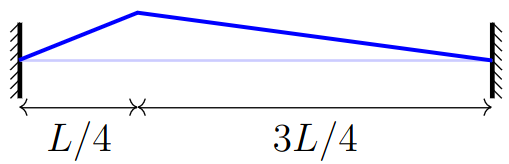
\includegraphics[width = 5.0in]{q2.png}
\end{center}
\begin{solution}
    We can see that this is a piecewise function woth two linear parts, one from $0<x<{L}{4}$ and the other from $\frac{L}{4}<x<L$. Let the height to which the string is plucked
    some value say $h$. So for the first part the function passes through the coordinates $({L}{4},h)$ and $(0,0)$, thus we have the function.    \begin{align*}
        & y = \cfrac{h}{{L}{4}} (x) \\ 
        \Rightarrow& y = \cfrac{4h}{L}x
    \end{align*}
    For the second part we have the line passing through the coordinates $(L/4,h)$ and $(L,0)$. Thus we have the function,
    \begin{align*}
        & y = \cfrac{h}{L/4-L}(x-L)\\ 
        \Rightarrow& y = -\cfrac{4h}{3L}(x-L)
    \end{align*}
    Thus we have the piecewise function definition
    \begin{equation*}
        f(x) =
        \begin{cases}
            \;\cfrac{4h}{L}x & \text{ if } 0<x<\cfrac{L}{4} \\
            -\cfrac{4h}{3L}(x-L)& \text{ if  } \cfrac{L}{4}<x<L
        \end{cases}
    \end{equation*}
    We need to show a fourier series representation of the above function. 
    \begin{align*}
        f(x) = a_0 + \sum_{n=1}^\infty a_n\cos\left(\cfrac{n\pi}{L}x\right) + \sum_{n=1}^\infty b_n\sin\left(\cfrac{n\pi}{L}x\right)
    \end{align*}
    $a_n = 0\ \ \forall n$ as the cosine terms do not become $0$ and thus do not satisfy the boundary conditions as the ends of the string are fixed and at $y=0$.
    we can take $a_0$ to be any value we want as that value in th physical scenario doesn't matter as the string is tied between two and ends and we can take one of the ends to
    be the origin without consequence. The $a_0$ is just a term that translates the whole fourier function graph upward or downward. We only need to find the 
    coefficients of the sine terms i.e. $b_n$. 
    \begin{align*}
        &\sum_{n=1}^\infty b_n \sin\left(\cfrac{n\pi x}{L}\right) = f(x) \\ 
        \Rightarrow&\sum_{n=1}^\infty b_n \sin\left(\cfrac{n\pi x}{L}\right)\sin\left(\cfrac{m\pi x}{L}\right) = f(x)\sin\left(\cfrac{m\pi x}{L}\right)\\
        \Rightarrow&\int^{L}_{0}\sum_{n=1}^\infty b_n \sin\left(\cfrac{n\pi x}{L}\right)\sin\left(\cfrac{m\pi x}{L}\right)dx = \int^{L}_{0}f(x)\sin\left(\cfrac{m\pi x}{L}\right)dx\\
    \end{align*}
    As we know that the integral picks out the $n^{th}$ value from the sum, thus giving us the coefficient $b_n$
    \begin{align*}
        \Rightarrow&\int^{L}_{0} b_n \sin^2\left(\cfrac{n\pi x}{L}\right)dx = \int^{L}_{0}f(x)\sin\left(\cfrac{m\pi x}{L}\right)dx\\
        \Rightarrow& b_n \cfrac{L}{2} = \int^{L/4}_0 \frac{4h}{3L}x\sin\left(\cfrac{n\pi x}{L}\right)dx - \int^L_{L/4}\frac{4h}{3L}(x-L)\sin\left(\cfrac{n\pi x}{L}\right)\\ 
        \Rightarrow& b_n = \cfrac{8h}{L^2}\left[\int^{L/4}_0x\sin\left(\cfrac{n\pi x}{L}\right)dx - \frac{1}{3}\int^L_{L/4}(x-L)\sin\left(\cfrac{n\pi x}{L}\right)\right]\\ 
        \Rightarrow & b_n = \cfrac{8h}{L^2}\left[ \frac{L^2}{{\pi}^2n^2}\sin\left(\frac{{\pi}nx}{L}\right)- \frac{L}{{\pi}n}x\cos\left(\frac{{\pi}nx}{L}\right)\Bigg|_{0}^{L/4} 
        -{1}{3}\left(\frac{L^2}{\pi^2n^2}\sin\left(\frac{{\pi}nx}{L}\right)+\frac{L}{\pi n}\left(L-x\right)\cos\left(\frac{\pi nx}{L}\right)\right)\Bigg|_{L/4}^{L}\right]\\ 
    \end{align*}
    Let us solve the intgrals piecewise : 
    \begin{align*}
        \tag{Part 1}
        \int^{L/4}_0x\sin\left(\cfrac{n\pi x}{L}\right)dx &=  \left[\left( {L^2}{{\pi}^2n^2}\sin\left(\frac{{\pi}nx}{L}\right)- \frac{L}{{\pi}n}x
            \cos\left({{\pi}nx}{L}\right)\right)\Bigg|_{0}^{L/4}\right]\\
                                                          & =\cfrac{L^2}{\pi^2 n^2}\sin\left(\cfrac{{\pi}n}{4}\right)-\cfrac{L^2}{4\pi n}\cos\left(\cfrac{\pi n}{4}\right)
    \end{align*}
    \begin{align*}
        \tag{Part 2}
        {1}{3}\int^L_{L/4}(x-L)\sin\left(\cfrac{n\pi x}{L}\right) &=\frac{1}{3}\left(\frac{L^2}{\pi^2n^2}\sin\left(\frac{{\pi}nx}{L}\right)+\frac{L}{\pi n}\left(L-x\right)\cos\left(\frac{\pi nx}{L}\right)\right)\Bigg|_{L/4}^{L}\\ 
                                                                       &= \cfrac{L^2}{3{\pi}^2n^2}\cdot\sin\left({\pi}n\right)-\cfrac{L^2}{3{\pi}^2n^2}\sin\left({{\pi}n}{4}\right)-\cfrac{L^2}{{4\pi}n}\cos\left(\frac{{\pi}n}{4}\right)\\
                                                                        \tag{since n$ \in \mathbb{N},\sin(n\pi) = 0$ }
                                                                       & =-\cfrac{L^2}{3{\pi}^2n^2}\sin\left({{\pi}n}{4}\right)-\cfrac{L^2}{{4\pi}n}\cos\left(\frac{{\pi}n}{4}\right)
    \end{align*}
    Part 1 + Part 2 = $b_n\cfrac{L^2}{8h}$
    \begin{align*}
        b_n &=\cfrac{8h}{L^2}\left[\cfrac{L^2}{\pi^2 n^2}\sin\left(\cfrac{{\pi}n}{4}\right)-\cancel{\cfrac{L^2}{4\pi n}\cos\left(\cfrac{\pi n}{4}\right)}+\cfrac{L^2}{3{\pi}^2n^2}\sin\left(\cfrac{{\pi}n}{4}\right)+\cancel{\cfrac{L^2}{{4\pi}n}\cos\left(\cfrac{{\pi}n}{4}\right)}\right]\\
            &=\cfrac{32h}{3L^2\pi^2n^2}\sin\left(\cfrac{n\pi}{4}\right) 
    \end{align*}
    Thus we have the Fourier series as 
    \fbox{ $f(x,t=0) = \sum^\infty_n  \cfrac{32h}{3L^2\pi^2n^2}\sin\left(\cfrac{n\pi}{4}\right) \sin\left(\cfrac{n\pi x}{L}\right)$}

\end{solution}
(b) Show that normal modes having nodes at L/4 are absent.
\begin{solution}
    The normal modes with a node at ${L}{4}$ are absent because $b_n$ vanishes. Physically it also makes sense as the amplitude of the string at $t=0$ is at $\frac{L}{4}$. We have 
    a node at ${L}{4}$ meaning $\sin\left(\frac{n\pi x}{L}\right)= \sin\left(\frac{n\pi L}{4L}\right)= \sin\left(\frac{n\pi}{4}\right)=0\Rightarrow n=4m$ for some $m\in\mathbb{N}$.
    So the whole normal mode
    \begin{align*}
        b_n &=  \cfrac{32h}{3L^2\pi^2n^2}\sin\left(\cfrac{4m\pi}{4}\right)\\ 
            &= \cfrac{32h}{3L^2\pi^2n^2}\sin\left(m\pi\right)\\
            \tag{$\sin(m\pi) =0~~\forall~~m\in\mathbb{N}$}
            &=0
    \end{align*}
    Thus the normal modes with nodes at $x=\cfrac{L}{4}$ vanish to 0.
\end{solution}
(c) Check numerically that your solution matches with the given shape. You may submit
your codes.
\begin{solution}
    \begin{lstlisting}[language = Python]
        import matplotlib.pyplot as plt
        import numpy as np
        L=np.pi
        h=np.e
        x = np.linspace(0,L,20000)
        x1 = np.linspace(0,L/4,5000)
        x2 = np.linspace(L/4,L,5000)
        y1 = (4*h/L)*x1
        y2 = -(4*h/(3*L))*(x2-L)
        def fourierfunc(x,n):
            y=0
            for i in range(1,n+1):
                y+= ((32*h/(3*i*i*np.pi*np.pi))*np.sin((np.pi*i)/4) * np.sin(i*np.pi*x/L))
            return y
        fig,axes = plt.subplots(figsize=(16,9),dpi=400,nrows = 2, ncols = 2)
        turns = [1,5,10,50]
        fig.suptitle("Fourier Series")
        for i in range(0,2):
            for j in range(0,2):
                axes[i][j].set_title(str(turns[2*i+j])+" Terms")
                axes[i][j].plot(x1,y1,lw = '2',color = "blue",label= "y = f(x) ")
                axes[i][j].plot(x2,y2,lw = '2',color = "blue")
                axes[i][j].plot(x, fourierfunc(x,turns[2*i+j]),color = "red",lw =2, label = "Fourier series upto "+str(turns[2*i+j])+" terms")
                axes[i][j].set_ylim([0,3.5])
                axes[i][j].set_xlim([0,np.pi])
                axes[i][j].legend(loc = "best")
                axes[i][j].grid()
    \end{lstlisting}
    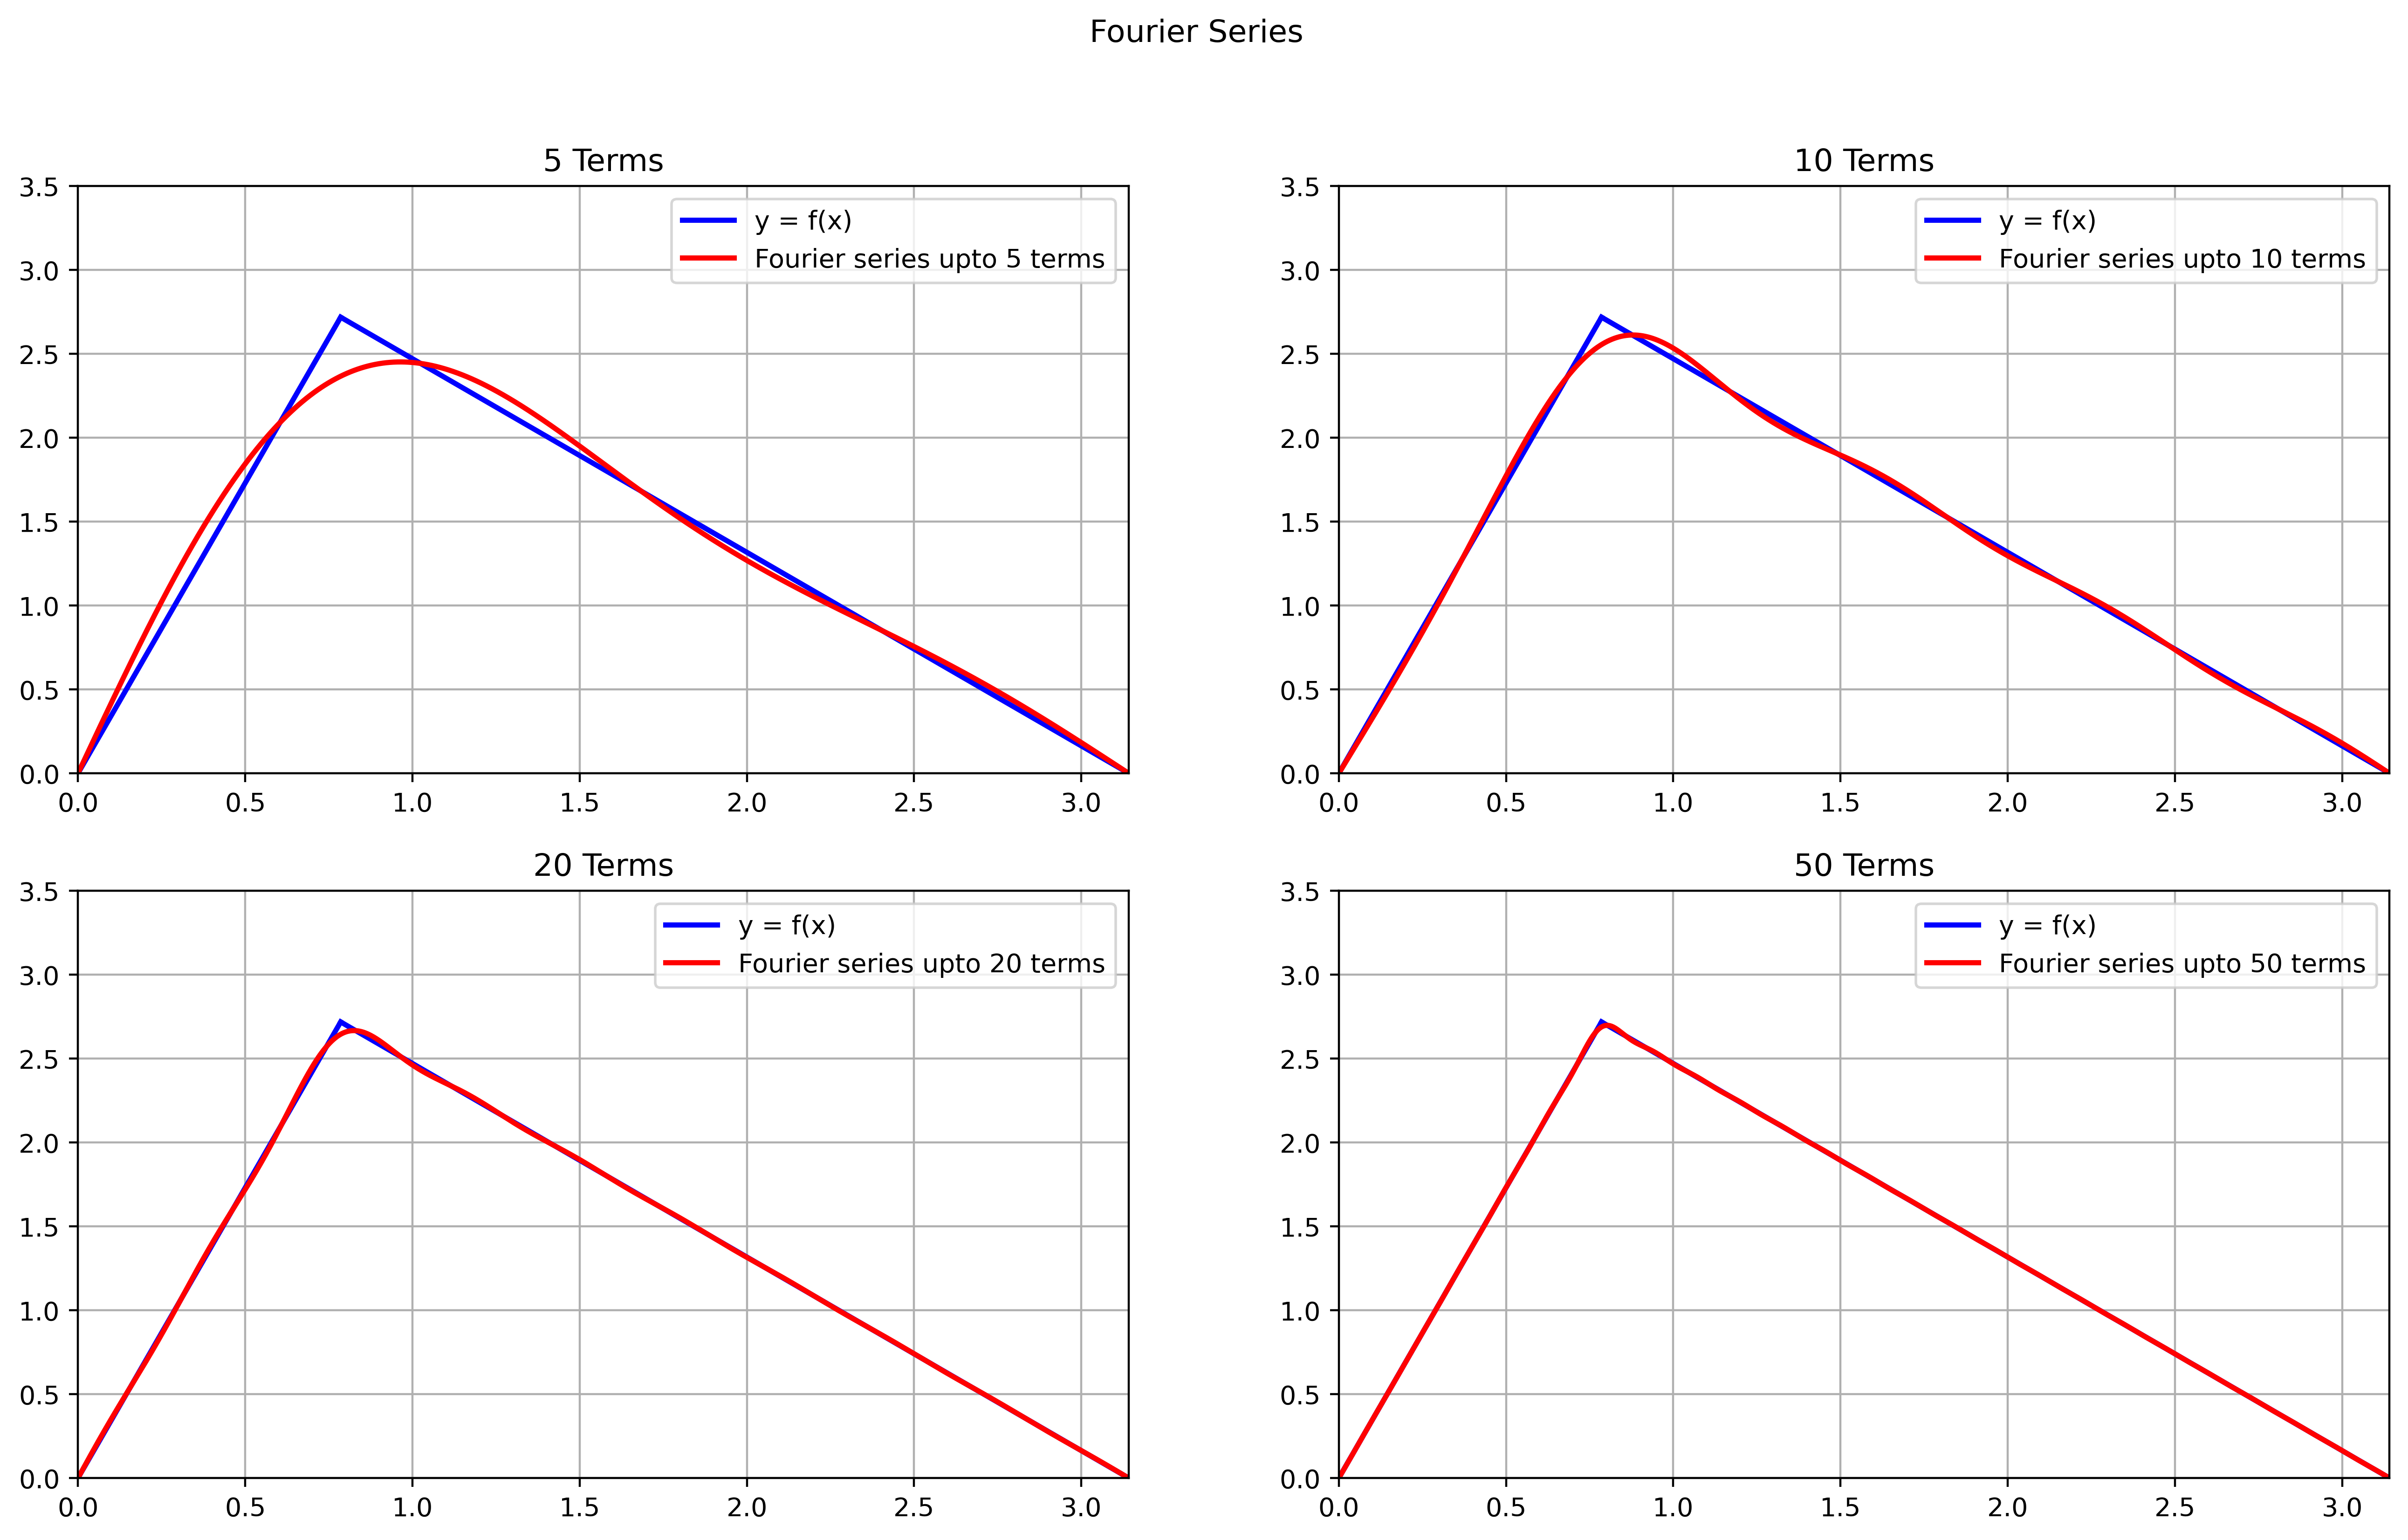
\includegraphics[width = 6.0in]{output_6_0.png}
\end{solution}
\newpage
\question \textbf{ Question 4}
Consider the following pattern. Find the Fourier representation of this pattern. Use the
complete representation (using sine and cosine). Also, check numerically that your solution
matches with the given shape. You may submit your codes.\\
\begin{center}
    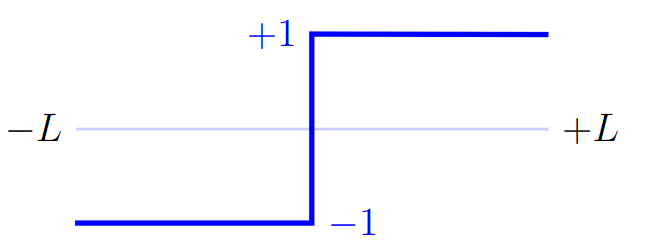
\includegraphics[width = 3.0in]{q4.png}
\end{center}
\begin{solution}
    \begin{align*}
        f(x) =
        \begin{cases}
            ~\ 1 & \text{if } -L<x<0 \\
            -1 & \text{if } 0<x<L
        \end{cases}
    \end{align*}
    The graphs plotted by the software are shown below.
    \begin{lstlisting}[language = python]
        import matplotlib.pyplot as plt
        import numpy as np
        L=np.pi*np.e
        x = np.linspace(-L,L,10000)
        x1 = [-L,0,L]
        y1 = [-1,-1,1]

        def fourierfunc(x,n):
            y=0
            for i in range(1,n+1,2):
                y = y + ((4/(i*np.pi))*np.sin(i*np.pi*x/L))
            return y
        fig,axes = plt.subplots(figsize=(16,16),dpi=400,nrows = 3, ncols = 2)
        turns = [5,10,20,50,100,200]
        fig.suptitle("Fourier Series")
        for i in range(0,3):
            for j in range(0,2):
                axes[i][j].set_title(str(turns[2*i+j])+" Terms")
                axes[i][j].axvline(0, color = 'black', lw = 2)
                axes[i][j].axhline(0, color = 'black', lw = 2)
                axes[i][j].step(x1,y1,lw = 3,color = "blue",label= "y = f(x) ")
                axes[i][j].plot(x, fourierfunc(x,turns[2*i+j]),color = "red",lw =2, label = "Fourier series upto "+str(turns[2*i+j])+" terms")
                axes[i][j].set_ylim([-1.5,1.5])
                labels = [item.get_text() for item in axes[i][j].get_xticklabels()]
                labels[1] = "L"
                labels[-2] = "-L"
                axes[i][j].set_xticklabels(labels)
                axes[i][j].legend(loc = "best")
                axes[i][j].grid()
    \end{lstlisting}
     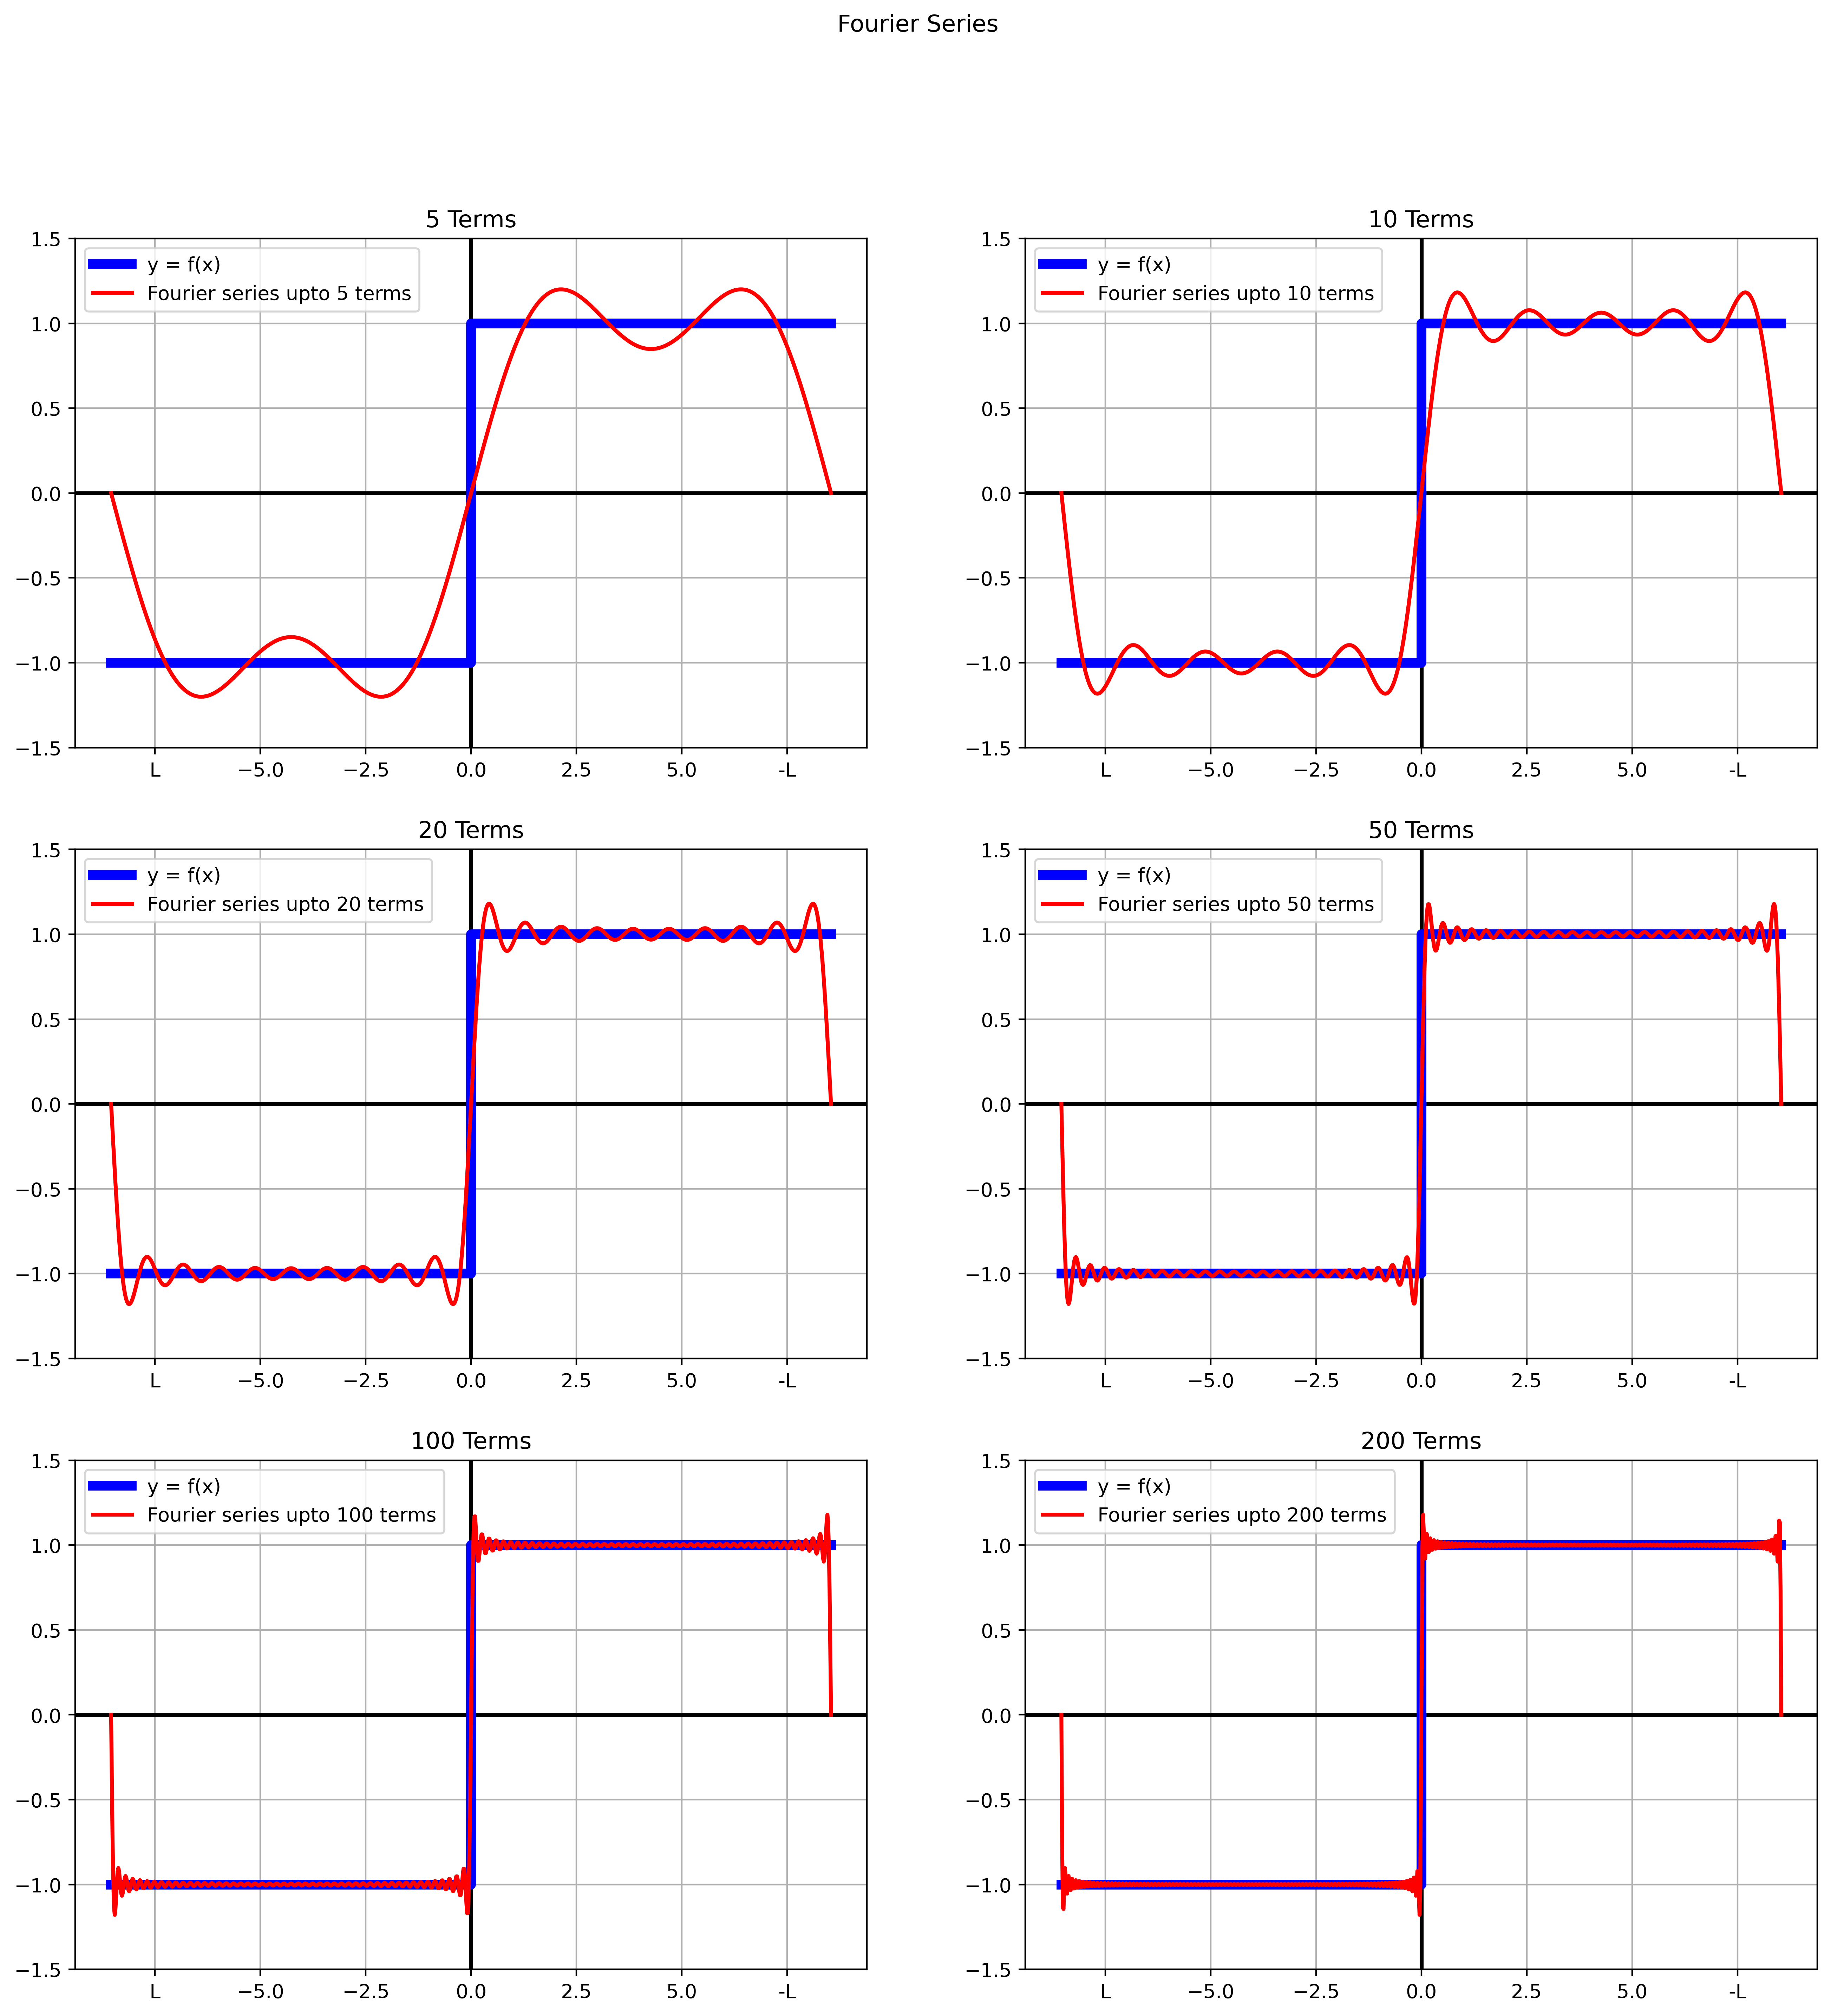
\includegraphics[width = 6.0in]{output_3_1.png}
\end{solution}

\end{questions}
\end{document}
